\documentclass[tikz,border=6mm]{standalone}
\usepackage{tikz}
\usepackage{xcolor}
\usetikzlibrary{arrows.meta,calc,decorations.pathmorphing,shapes.geometric,positioning,backgrounds,fit,shadings,patterns}
\definecolor{substblue}{RGB}{70,130,180}
\definecolor{procamber}{RGB}{180,110,30}
\definecolor{feltgreen}{RGB}{0,110,55}
\definecolor{bgcream}{RGB}{252,248,240}
\definecolor{atomblue}{RGB}{100,160,210}
\definecolor{emphred}{RGB}{160,40,40}
\definecolor{panelborder}{RGB}{180,170,155}

\begin{document}
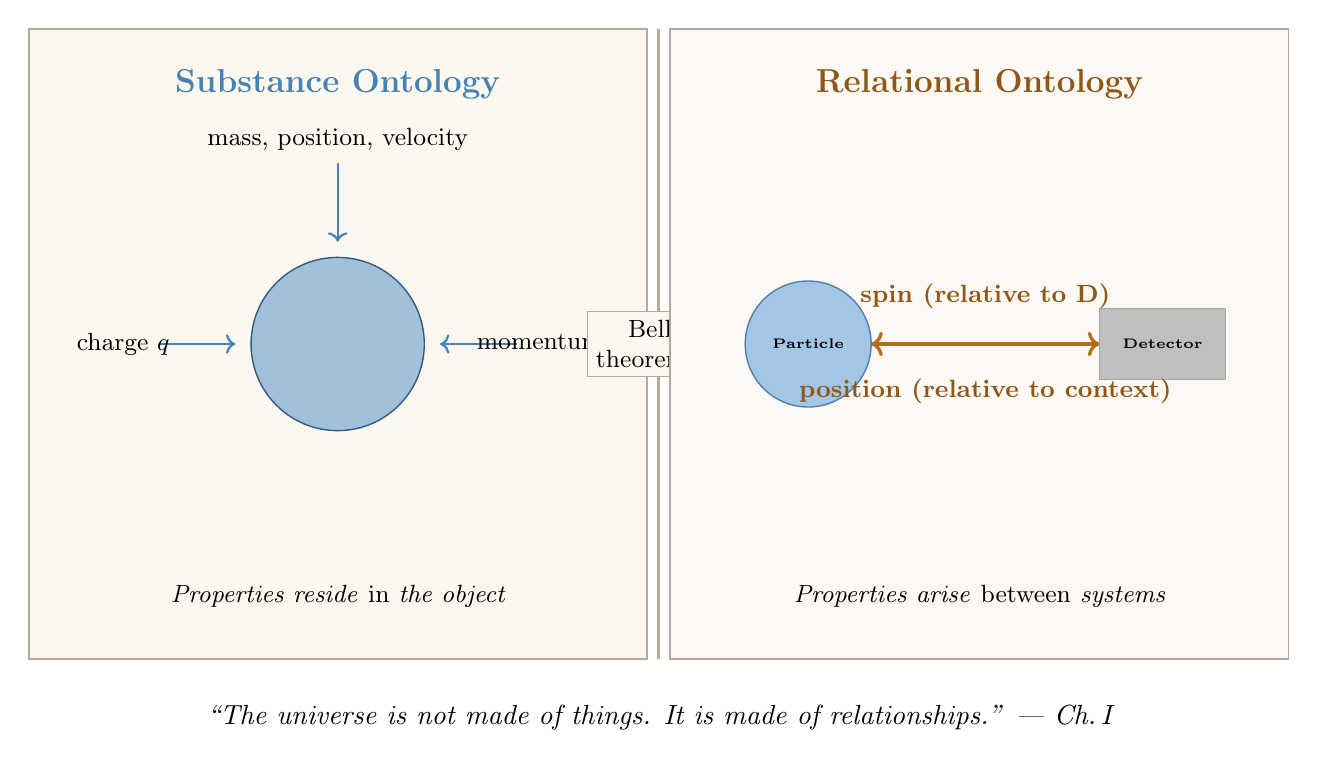
\begin{tikzpicture}[
  every node/.style={font=\sffamily},
  inward/.style={->, thick, substblue, shorten >=2mm},
  relational/.style={<->, very thick, procamber},
]

% ===== Overall dimensions =====
% Left panel: x in [-8, -0.15], right panel: x in [0.15, 8], y in [-4, 4]
% Caption strip below: y in [-5, -4.2]

%% ---- LEFT PANEL: Substance Ontology ----
\fill[bgcream, draw=panelborder, line width=0.7pt]
  (-8.0,-4.0) rectangle (-0.15, 4.0);

% Panel title
\node[substblue, font=\bfseries\large, align=center] at (-4.075, 3.3)
  {Substance Ontology};

% Billiard ball
\fill[substblue!50, draw=substblue!70!black, line width=0.5pt]
  (-4.075, 0) circle (1.1cm);

% Arrow: top → ball (from y=2.4 down to ball edge)
\draw[inward] (-4.075, 2.3) -- (-4.075, 1.1);
\node[align=center, font=\small] at (-4.075, 2.6)
  {mass, position, velocity};

% Arrow: right → ball
\draw[inward] (-1.8, 0) -- ({-4.075+1.1}, 0);
\node[align=center, font=\small] at (-1.35, 0)
  {momentum $\mathbf{p}$};

% Arrow: left → ball
\draw[inward] (-6.35, 0) -- ({-4.075-1.1}, 0);
\node[align=center, font=\small] at (-6.8, 0)
  {charge $q$};

% Panel caption
\node[font=\itshape\small, align=center] at (-4.075, -3.2)
  {Properties reside \emph{in} the object};

%% ---- CENTER DIVIDER ----
\draw[panelborder, line width=1.0pt] (0,-4.0) -- (0, 4.0);

% Bell's theorem label on divider
\node[draw=panelborder, fill=bgcream, font=\small, inner sep=3pt,
      align=center] at (0, 0)
  {Bell's\\theorem $\rightarrow$};

%% ---- RIGHT PANEL: Relational Ontology ----
\fill[bgcream!80!procamber!20, draw=panelborder, line width=0.7pt]
  (0.15,-4.0) rectangle (8.0, 4.0);

% Panel title
\node[procamber!80!black, font=\bfseries\large, align=center] at (4.075, 3.3)
  {Relational Ontology};

% Particle circle (left side of right panel)
\fill[atomblue!60, draw=atomblue!80!black, line width=0.5pt]
  (1.9, 0) circle (0.8cm);
\node[font=\tiny\bfseries, align=center] at (1.9, 0) {Particle};

% Detector rectangle (right side of right panel)
\fill[gray!50, draw=gray!70, line width=0.5pt]
  (5.6,-0.45) rectangle (7.2, 0.45);
\node[font=\tiny\bfseries, align=center] at (6.4, 0) {Detector};

% Double-headed arrow between particle edge and detector left edge
\draw[relational] (2.7, 0) -- (5.6, 0);

% Label above arrow
\node[procamber!80!black, font=\small\bfseries, align=center] at (4.15, 0.6)
  {spin (relative to D)};

% Label below arrow
\node[procamber!80!black, font=\small\bfseries, align=center] at (4.15,-0.6)
  {position (relative to context)};

% Panel caption
\node[font=\itshape\small, align=center] at (4.075,-3.2)
  {Properties arise \emph{between} systems};

%% ---- BOTTOM CAPTION (below whole figure) ----
\node[font=\itshape, align=center] at (0,-4.75)
  {``The universe is not made of things. It is made of relationships.'' --- Ch.\,I};

\end{tikzpicture}
\end{document}
